% This is samplepaper.tex, a sample chapter demonstrating the
% LLNCS macro package for Springer Computer Science proceedings;
% Version 2.20 of 2017/10/04
%
\documentclass[runningheads]{llncs}
%
\usepackage{graphicx}
\usepackage{subcaption}
\usepackage{float}
\usepackage{todonotes}
\usepackage{amsmath}
% Used for displaying a sample figure. If possible, figure files should
% be included in EPS format.
%
% If you use the hyperref package, please uncomment the following line
% to display URLs in blue roman font according to Springer's eBook style:
% \renewcommand\UrlFont{\color{blue}\rmfamily}

\begin{document}
%
\title{Embedded Reachability for Half the Price\thanks{Supported by organization x.}}
%
%\titlerunning{Abbreviated paper title}
% If the paper title is too long for the running head, you can set
% an abbreviated paper title here
%
\author{Nathan Jewell\inst{1}\orcidID{0000-1111-2222-3333} \and
Stanley Bak\inst{2}\orcidID{2222--3333-4444-5555} \and
Houssam Abbas\inst{1}\orcidID{1111-2222-3333-4444}} 
%
\authorrunning{N. Jewell et al.}
% First names are abbreviated in the running head.
% If there are more than two authors, 'et al.' is used.
%
\institute{Oregon State University, Corvallis OR 97333, USA \and
\email{jewelln@oregonstate.edu}}
\institute{Stony Brook University, USA \and
\email{jewelln@oregonstate.edu}}
%
\maketitle              % typeset the header of the contribution
%
\begin{abstract}
This paper demonstrates that it is possible to obtain accurate, real-time reachability computations for an autonomous vehicle using only simple kinematics, parallelization on a GPU without any algorithmic changes, and while running a full autonomous racing stack.
This stands in contrast to existing work which required the development of custom parallelizable reachability algorithms, the use of accurate nonlinear models of the dynamics, and was limited to a shorter look-ahead horizon. 
Reachability analysis enables the safety assurance of control systems despite uncertain initial conditions and control inputs, and can be an important component to run on-board an autonomous system.
%The runtime of reachability analysis depend on the the system dynamics, the reachability algorithm, the hardware it is running on, and what other processes are sharing the hardware.
%
In this work we set out to see whether it is possible to obtain accurate and timely reachability computations using a common CPU+GPU hardware on-board an autonomous vehicle, with minimal upfront effort.
We leverage HYLAA, a state-of-the-art reachability tool.
Our solution uses simple linearized kinematics, yet it is accurate; runs in Python, yet is real-time; shares the hardware with a full autonomous racing stack including a state-of-the-art optimization-based predictive controller; and is partitioned between CPU and GPU without any algorithmic modifications, rather, only code-level parallelization is used.
In our testing we achieve accurate 10-step reachability as quickly as 150 milliseconds. We also find that porting portions of reachability onto the GPU can improve the runtime for 10-step reachability by 62\% over a CPU only implementation.% and reduces the computational complexity in relation to number of reachability steps.
We demonstrate our results on the F1/10 1/10th-scale autonomous race car.
This work lowers the barrier to running reachability significantly, as it removes the need to do time-consuming system identification, the need to employ nonlinear reachability tools, and the need to do an algorithm-specific modifications to enable GPU parallelization.

\keywords{Reachability  \and Safety Analysis \and CUDA \and GPU}
\end{abstract}
%
%
%
\section{Introduction}
Reachability is the computation and interpretation of possible future agent states at a time or set of times. Given an agent's current state and a range of possible future inputs, a reachability algorithm outputs information about all possible states of the agent at time $T$ in the future. For computational efficiency and practical use, we discuss discrete-time reachability algorithms. In discrete-time reachability, a range of $N$ possible state spaces are generated for $N$ future times. defined by intervals spaced by the discretization time step, $dt$. Importantly the generated state spaces are minimal overapproximations of possible states as defined by the agent’s dynamical model. This guarantees that any state actually reached at time $T$ is within the overapproximation boundary and can be utilized for safety analysis.

Safety verification is the overarching goal for reachability computations. With highly reliable systems, it is necessary to verify that no error state could be reached. In autonomous vehicles, error states may involve intersections with walls, other cars or people, etc.. By checking the overapproximation of states, it can be determined if the agent is in danger of reaching an error mode in the future. Planned inputs can then be modified to avoid the danger, preventing potentially catastrophic system failure.

We explore a number of different runtime modes for profiling successively linearized reachability computation. These modes are chosen to stress different components of the host system, improve runtime, and demonstrate the effectiveness of real time safety analysis alongside real-world loads.

\section{Background}
\subsection{F1/10 Platform}
The F1/10 autonomous racing platform is a standardized hardware platform designed to facilitate algorithmic improvements for high-reliability autonomous systems. The vehicle consists of a highly modified one tenth scale remote control chassis and is equipped with an improved electronic speed controller and lidar. The compute platform is an NVIDIA Jetson TX2 computer designed for use in embedded systems. The Jetson TX2 is equipped with a dual CPU setup providing 6 physical cores onboard the vehicle as well as a modern NVIDIA GPU and 8GB RAM. The installed autonomous navigation and mapping software is a combination of low-level nodes to interface with hardware, publicly available SLAM algorithms, and the model predictive control and reachability sofware developed in our lab.




\subsection{The HYLAA Tool}
The original HYLAA tool allows for solving linear reachability problems represented by hybrid automata with affine dynamics. HYLAA output is defined as a collection of reach sets. A reach set is the approximation of all possible \emph{reachable} states at future time $t$. HYLAA adopts a simulation-equivalent approach where the superposition principle for linear systems is applied to reduce the number of necessary simulations for any mode to $N+1$ for each simulated step in a N-dimensional system. Safety conditions represented by their linear inequalities are evaluated inline with the simulation and a variety of condition 
Basic definition of reach set, how HYLAA works (one paragraph)

\subsection{QuickZono: a HYLAA variant}
Quickzono simplifies the HYLAA algorithm, opening the possibility of realtime performance. Many features of HYLAA were secondary to generating the core set of reachable states and could be removed to improve performance. Instead of using the formalism of hybrid automata, QuickZono uses zonotopes to represent the agent state and perform the reachability simulation. The agent state at time $t$, $S_t$ is used to compute the next reachable set $S_{t+dt}$ at time $t + dt$ where $dt$ is the discretization step-size. The computation is in the form $S_{t+dt} = S_t \cdot A + I_t \cdot B$ where $I_t$ is the planned inputs at time $t$ and matrices $A, B$ are the dynamics for the system linearized around the predicted agent state given by the MPC. Quickzono also leaves the checking of safety conditions for post-processing step, but importantly still produces 2-dimensional projections necessary for validating these conditions in linear time.

\subsection{Successively Linearzied Kinematics}
We identified a simple 3 variable kinematic model for the car based on its physical properties.
\begin{align}
\dot{x} = v \cos{\psi + d} \\
\dot{y} = v \sin{\psi + d} \\
\dot{\psi} = v \frac{1}{L} \sin(d)
\end{align}

According to the underlying algebra of the reachability computation in HYLAA and Quickzono, $S_{t+dt} = S_t \cdot A + I_t \cdot B$, linear dynamics were computed for matrices $A_t$ and $B_t$ for state $S_t$

Take a nonlinear equation $g(c)$ By definition, the linearization for g, $L_g(c)$ around a point $\bar{c}$ is given by

$$L_g(c) = g(\bar{c}) + g'(\bar{c})(c-\bar{c})$$

Applied to the algebra for reachability this equates
\susection{Parallelizing Reachability}
Initial profiling of Quickzono using pycallgraph and cProfile revealed the large portion of computation time was spent projecting from n-dimensional zonotopes onto the useful 2-dimensional polygons which can be used to analyze safety parameters in the lower dimensional agent environment. So, this projection step was chosen as the most impactful target for parallelization. The projection was particularly well suited for this because the algorithm depends only on the target zonotope and thus is trivial to parallelize across all outputed zonotopes on the CPU.

GPU parallelization using CUDA was then written using a direct translation for the most time intensive function called recursively in the projection algorithm. A rudimentary strategy for parallelization was applied which directly translated the iterative CPU code into a single CUDA Kernel. Effort was taken to minimize the number of memory copies to and from the GPU and GPU compute resources were dynamically allocated depending on the number of vertices being considered in that particular projection step as well as the dimensionality of the reachability problem.

\section{Experimental Setup}


\subsection{Runtime Modes}

\subsubsection{HYLAA} \newline The original hybrid reachability tool [cite].
\vspace*{-5pt}
\subsubsection{Quickzono Single Core} [QZ\_CPU] \newline A simplified subset of HYLAA code with succinct wrappers. 
\vspace*{-5pt}
\subsubsection{Quickzono Multiple Core} [QZ\_MP] \newline Quickzono code with a trivial CPU-based multiprocessing model \newline applied to the projection step. 
\vspace*{-5pt}
\subsubsection{Quickzono GPU Hybrid} [QZ\_HYBRID] \newline Hybrid GPU/CPU implementation, with the most taxing\newline part of the projection algorithm moved onto the GPU device. 
\vspace*{-5pt}

\subsection{Profiling Reachability Within the Stack}

In \textit{offline} profiling, reachability is computed as the sole program running on the system. A dedicated testing script executes each of the runtime modes for 200 trials at intervals between 4 and 24 reachability steps. HYLAA is only tested over 5 trials due to slow performance. 
The script outputs timing data excluding any one-off setup and configuration code.

In \textit{online} profiling, reachability is computed as part of a ROS network running physical control nodes (controller input, motor and servo control, etc.), a GPU-based particle filter node for localization, a model predictive control node, and various other supporting nodes. 
Before beginning the profiling, the vehicle is placed into the test track, localized and configured to autonomously drive the track until profiling is complete. 
The reachability node is implemented as a wrapper for the various reachability modes described above and records call timings for the same function, executing as quickly as possible. 
The online profiler is configured to automatically switch between runtimes modes and vary the number of reachability steps. This occurs for the same parameters as in offline profiling, except that only those configurations executing at least 4hz (<=250ms per trial) are considered. Full HYLAA is not tested in this profiling due to slow performance.

\subsection{Performance Characteristics}
There are a number of important characteristics needed to describe the performance of a real time embedded algorithm.

Correctness means that the outputs are a valid solution to the problem, namely that the computed set is indeed a reachset for the dynamics.

Scalability is how well the algorithm scales with increasing problem size. In our case, problem size is measured by the number $N$ of time steps. The number of steps is increased either by an increase in horizon $T$ or a decrease in discretization step-size $dt$, or both: $T$ = $N\cdot dt$. It is important to understand how the algorithm scales so intelligent decisions can be made about optimal horizon and precision in real time applications.

Runtime is the time to solve the given problem. 
Running a safety algorithm is only effective when there is a low latency between consecutive executions. If this criterion is not met, safety analysis could be out of date when the agent is developing a response, resulting in ineffective performance or a collision. 
In contrast, low latency [runtime] will improve the safety margin of the agent by providing reachability information to the controller early enough to develop a response to it.

Runtime variability is the standard deviation in the runtime. While latency is of primary importance, the consistency of the tool's runtime is paramount for autonomous systems. 
Latency spikes at the wrong time could create dangerous problems for the agent when reacting to unsafe conditions. 

\section{Methods}
\subsection{Collected Data}
Each characteristic has an empirical measure which we can use to analyze it quantitatively. Our offline and online profiling are run separately to evaluate the impact of running the reachability along with localization and control algorithms.

To validate correctness, we used HYLAA model output, assuming that HYLAA is mathematically consistent. Outputs from other runtime modes are compared to the HYLAA output to determine if there are any significant differences. It is not necessary to validate correctness separately for online and offline computation since the same code is executed in each case.

To validate scalability, each runtime model is tested with a range of values for the number of reachability steps which are representative of useful workloads. The number of steps, $N$ is equal to the ratio between total horizon time in seconds, $T$ and the discretization time-step $dt$. This varying of step values is done for both online and offline modes. However, for online trials, only models capable of running around 250ms per iteration (4hz) are considered.

To test runtime, each combination of runtime mode and steps is evaluated over multiple trials. The recorded runtimes will be the average over 200 trials. This data collection is done for both online and offline testing.

To test runtime variability, the all recorded runtimes from all trials are analyzed. We compute standard deviation in runtime and 95\% runtime confidence intervals around the mean assuming normally distributed variation in runtimes. This analysis is performed for both online and offline testing.

Some other values are also collected for the benefit of running analysis. 
What is a trial? One execution of the reachability computation.  


\section{Results}

\begin{figure}[t]
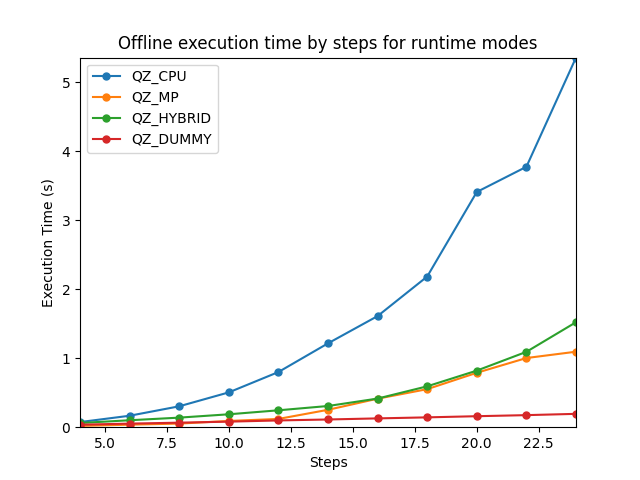
\includegraphics[width=\textwidth]{profiler_out/offline_avg_unified.png}
\caption{Average Offline trial execution times for all runtime modes.} \label{offline_avg}
\end{figure}

\begin{figure}[t]
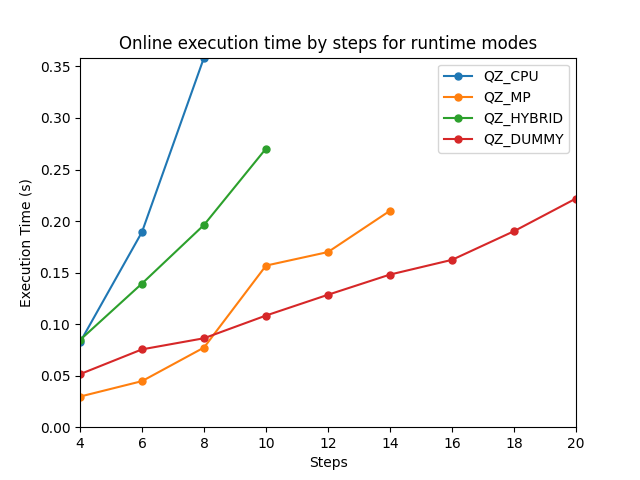
\includegraphics[width=\textwidth]{profiler_out/online_avg_unified.png}
\caption{Average Online trial execution times for all runtime modes.} \label{online_avg}
\end{figure}
\begin{figure}[t]
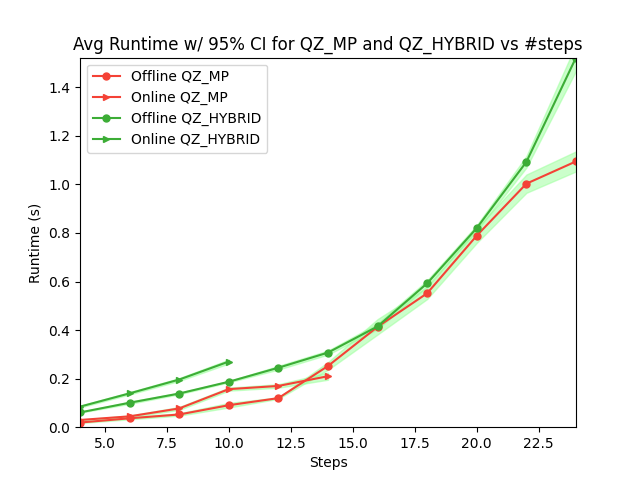
\includegraphics[width=\textwidth]{profiler_out/avg_mp_hybrid_CI.png}
\caption{Comparison between Multiprocessing and Hybridized online and offline runtimes.} \label{mp_hybrid_ci}
\end{figure}
\begin{figure}[t]
    \subcaptionbox{Detail of the Quickzono GPU Hybrid runtimes with 95\% confidence intervals.\label{CPU_CI}}{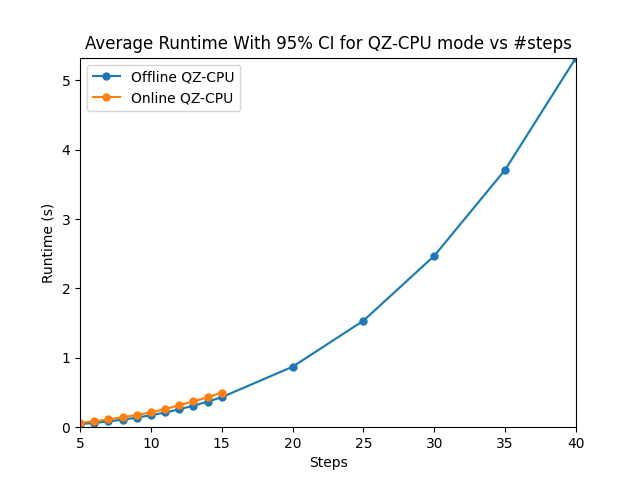
\includegraphics[width=.5\linewidth]{profiler_out/avg_QZ-CPU_CI.png} }
    \subcaptionbox{Detail of the Quickzono Single Core runtimes with 95\% confidence intervals.\label{MP_CI}}{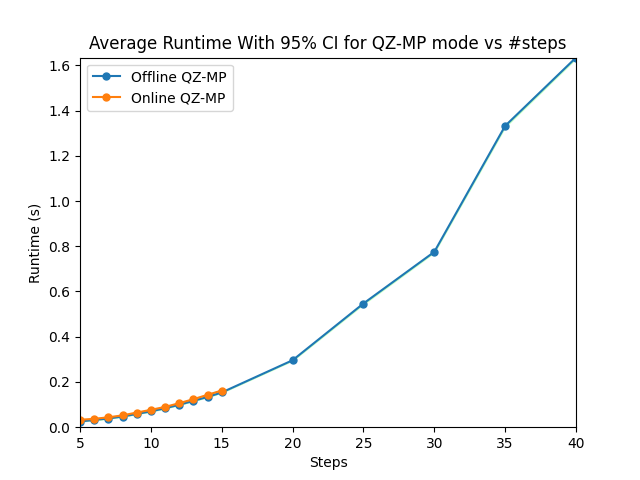
\includegraphics[width=.5\linewidth]{profiler_out/avg_QZ-MP_CI.png} }
\begin{subfigure}{\linewidth}
    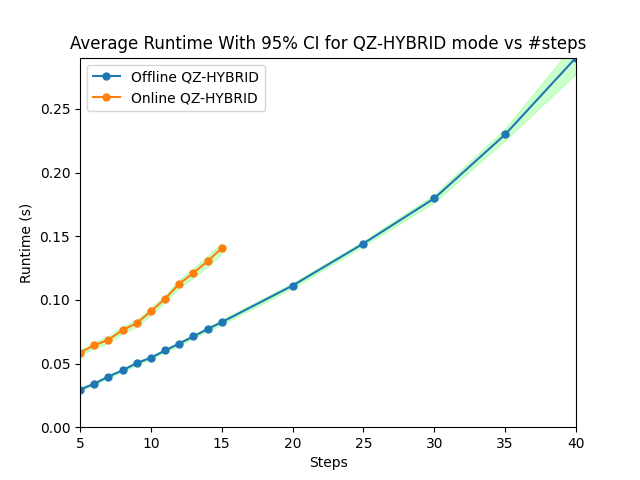
\includegraphics[width=.5\linewidth]{profiler_out/avg_QZ-HYBRID_CI.png}
    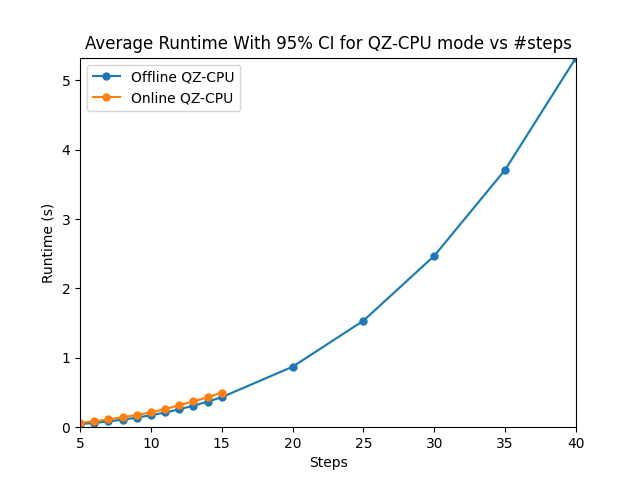
\includegraphics[width=.5\linewidth]{profiler_out/avg_QZ-CPU_CI.png} \hfill

\end{subfigure}

\end{figure}

\subsection{Discussion}

For offline timings, modes QZ\_CPU and QZ\_HYBRID \ref{offline_avg} show a pattern of exponential style growth. QZ\_DUMMY breaks this trend as we would expect since it is not doing meaningful computations for the zonotope projection algorithm which is the primary source of computational complexity. There is a reduction in runtime from CPU mode to QZ\_MP and QZ\_HYBRID modes indicating a that attempts at parallelization by various methods had useful impacts on the algorithms speed.

Both QZ\_HYBRID and QZ\_MP are capable of running realtime reachability effectively. 

Online execution times show less clear patterns since it is harder to infer from the fewer data points collected. 

%
% ---- Bibliography ----
%
% BibTeX users should specify bibliography style 'splncs04'.
% References will then be sorted and formatted in the correct style.
%
% \bibliographystyle{splncs04}
% \bibliography{mybibliography}
%
\begin{thebibliography}{8}


\bibitem{ref_hylaa}
Bak S., Sridhar Duggirala P.: HyLAA: A Tool for Computing Simulation-Equivalent Reachability for Linear Systems. In: Editor,
Proceedings of the 20th International Conference on Hybrid Systems: Computation and Control 2017

%@article{Bak2017HyLAAAT,
%  title={HyLAA: A Tool for Computing Simulation-Equivalent Reachability for Linear Systems},
%  author={Stanley Bak and Parasara Sridhar Duggirala},
%  journal={Proceedings of the 20th International Conference on Hybrid Systems: Computation and Control},
%  year={2017}
%}
\bibitem{ref_oder}
Maler O.: Computing Reachable Sets : An Introduction. 2008
%@inproceedings{Maler2008ComputingRS,
%  title={Computing Reachable Sets : An Introduction},
%  author={O. Maler},
%  year={2008}
%}
@inproceedings{DBLP:conf/hvc/RayGDBBG15,
  author    = {Rajarshi Ray and
               Amit Gurung and
               Binayak Das and
               Ezio Bartocci and
               Sergiy Bogomolov and
               Radu Grosu},
  editor    = {Nir Piterman},
  title     = {XSpeed: Accelerating Reachability Analysis on Multi-core Processors},
  booktitle = {Hardware and Software: Verification and Testing - 11th International
               Haifa Verification Conference, {HVC} 2015, Haifa, Israel, November
               17-19, 2015, Proceedings},
  series    = {Lecture Notes in Computer Science},
  volume    = {9434},
  pages     = {3--18},
  publisher = {Springer},
  year      = {2015},
  url       = {https://doi.org/10.1007/978-3-319-26287-1\_1},
  doi       = {10.1007/978-3-319-26287-1\_1},
  timestamp = {Sat, 19 Oct 2019 20:27:11 +0200},
  biburl    = {https://dblp.org/rec/conf/hvc/RayGDBBG15.bib},
  bibsource = {dblp computer science bibliography, https://dblp.org}
}
\end{thebibliography}
\end{document}
